\documentclass[12pt,letterpaper]{article}
\usepackage[left=2.6cm,top=2.5cm,right=2.6cm,bottom=2.5cm]{geometry} 
\usepackage[english]{babel}
\usepackage[utf8x]{inputenc}
\usepackage{amsmath}
\usepackage{eqnarray}
\usepackage{mathtools}
\usepackage{amssymb} 
\usepackage[retainorgcmds]{IEEEtrantools}
\usepackage{booktabs,caption}
\usepackage[flushleft]{threeparttable}
\usepackage{graphicx}
\usepackage{caption}
\usepackage{tabularx}
\usepackage{subfig}
\usepackage{kpfonts}    % for nice fonts
\usepackage{microtype} 
\usepackage{booktabs}   % for nice tables
\usepackage{bm}         % for bold math
\usepackage{listings}   % for inserting code
\usepackage{verbatim}   % useful for program listings
\usepackage{color}  
%\usepackage[colorlinks=true]{hyperref}%%TABLE % use for hypertext
\usepackage[colorlinks = true,
            linkcolor = blue,
            urlcolor  = blue,
            citecolor = blue,
            anchorcolor = black]{hyperref}
\usepackage[colorinlistoftodos]{todonotes}
\usepackage{natbib}
\renewcommand{\baselinestretch}{1.5}



\begin{document}

%+Title
\title{\LARGE{The effect of house prices on long term care market: Evidence from England}}
\author{Eduardo Gonzalo Almorox\thanks{Newcastle University Business School. 5 Barrack Rd, Newcastle upon Tyne NE1 4SE} \thanks{Corresponding author: \tt{e.gonzalo-almorox@newcastle.ac.uk} } \and Nils Braakmaann\footnotemark[2]
 \and Volodymyr Bilotkach\footnotemark[2] \and John Wildman\footnotemark[2]}


\date{First version: January 2017\\ This version: March 2017}
\maketitle

\begin{abstract}
This study investigates the effects of house prices in the English care homes market. 
High house prices, as experienced currently in England, may disincentive the entry in
 certain markets restricting the access to long term care services in these areas. Alternatively, 
 these areas may also suppose business opportunity. We provide evidence in order to disentangle 
 these effects. Considering the variation of the planning regulations accross English planning authorities for addressing
 potential endogeneity, our instrumental variables estimates suggest that higher house prices lead to an increase of the distribution of care homes. 
 These findings contribute to inform policy makers about the relationship between the long term care and housing markets. 
\end{abstract}

{{\bf{Keywords}}: Care homes, house prices, long-term care, England\\
\bf{JEL}: R31, I12}

\newpage
\tableofcontents
%\newpage
%-Title


\newpage
\section{Introduction}
\label{sec: intro}

England has experienced the fastest growth in house prices amongst all OECD country during the last decades.
This inflationary trend has had consequences for both households, materialised in the so called “house affordability crisis”, 
and to less extent businesses. In this paper we investigate the relationship between the house prices 
and the market structure of an industry that typically operates with low margins, the care homes 
that provide long term care services. Our interest in the long term care is not trivial. Elements such as 
the ageing of the population or some socioeconomic changes that include the inclusion of more women 
in the labour force as well as the composition of different family structures, have shifted informal caregiving 
towards more formal long term care provision. These patterns evidence the importance of this sector in the 
forthcoming decades. Yet, despite the will of policy makers to design policies that preserve a sustainable 
provision of long term care and that also ensure competitive market structures, there is limited evidence for
 the design of these policies.  We aim at informing these policies by analysing the extent of the effect of high 
 prices in the housing market on the entries in the market of care homes. 

The way high prices in the housing market may affect the local long term care markets is a priori uncertain 
as there are two opposing effects that may appear. The first may consist of the effect of house price 
as a cost for running a care home. Hence, higher house prices may suppose an important barrier that can restrict the
 entry in certain local markets. Furthermore, higher house prices may increase the opportunity costs of alternative
 building projects and therefore suppose an incentive to deter potential development of care homes. 
 A potential consequence derived from the former situations could be that people living in
  these areas may find less long term care choices closer to them. 
  
  The second existing effect may be derived from the the basis of how high house prices may represent
   a business opportunity. The segment of the population that benefits from current upward trend in the house
    prices are those elderly homeowners that are able to monetize the higher value of their asset by selling their
     houses and moving out cheaper areas \citep{hilber2016housingpolicies}. If this argument holds, areas with higher 
     prices may be associated with greater levels of affluence and consequently greater proportions of clients
      that are more willing to pay for the services of a care home. Although the latter may contribute to preserve 
      the financial viability of care homes in the market, an issue that constitutes a current public policy concern, 
      it may also result in an unequal distribution of long term care across different areas in England where the
       most affluent areas are more benefited from a greater supply of home care services. 

In order to proceed with our analysis, we construct a unique dataset that merges information from several 
sources to collate information regarding the characteristics of the dynamics in the care homes market, the
 housing markets and the planning regulations. The dataset captures information regarding local authorities 
 at different level (e.g. street, district and county level). A first technical hurdle concerning the dataset, consists
  of distinguishing de novo entries associated with providers that effectively produce a new activity. Secondly, 
  there is an additional empirical caveat that we have to address with regards to effect of house price on care
   homes entries. It may be possible that care homes select markets that have high prices on a non-random 
   basis due to unobservable variables. This sample selection bias may invalidate the estimates corresponding
    to the effects of house prices. In order to overcome these, we carry out and identification strategy which 
    uses an instrumental variables approach that exploits the variability in the restrictiveness of planning
     regulations across English districts. Our identification relies on the assumption that changes in the planning
      requirements affect the entry of care homes in market through the levels of house prices. 
      
To the best of our knowledge, no previous studies have been undertaken to provide causal evidence with
 regards to the effects of housing prices in the context of entries in the market of care homes. This research
  also makes a number of contributions to several strands of the literature. It provides further evidence to the 
  growing literature that analyses aspects associated with the market of care homes in England. \citet{forder2014} study the elements that determine the competition amongst care homes and assess the 
  consequences of this competition in both prices and quality. Also \citet{allan2015} evaluate empirically 
  the causes of market exits by investigating the effects of maintaining minimum standards in the quality of 
  the service. We extend this literature by addressing issues referred to the entry of care homes in the market. 
  Prior to this paper, only \cite{machin2003} have provided empirical evidence of factors affecting the market
   entry by analysing the effects of setting of a minimum wage. In addition to providing a more up to date
    evidence, this research uses a more extensive dataset provided by the regulator, the
     Care Quality Commission (CQC). Likewise, this research also extends the literature that studies the effects 
     of the planning system and the high house prices in England using the care homes as a new sector
      for the analysis. 
      
  \section{Institutional background}
  
  In England planning and long term care are activities that are ruled and applied by local governments. 
The structure of these is nonetheless complex and entails different organizational levels\footnote{These levels or tiers include three main groups: (i) county councils, (ii) district, borough or city councils and (iii) parish or 
town councils. Most of the activities designed by local governments are developed at county or district level 
(group (i) or (ii))} depending on the type of services that are regulated. 
In this section we outline the main characteristics of the local government in England 
considering the particular cases of planning regulations and long term care. 
This will help to understand the geography that we adopting for our empirical analysis. 
 
 England has 152 local authorities that operate at council level\footnote{The Health and Social Care Act (2008) 
supposed the transfer of public health matters from Primary Care Trusts (PCT) Clinical issues were responsibility of the clinical commissioning groups (CCG).} 
and have responsibilities on long term care through the commissioning – e.g. purchase of services.
 Since the mid-eighties, market mechanisms drive the provision of long term care services. The supply is mainly composed by private  \textit{for profit} providers and 
their distribution is quite unbalanced.  About the 15\% of market share is 
  concentrated in 4 “main providers” and the remaining 70\% of the market share is composed by providers 
  that have a reduced number of beds - no more than 0.4\% of the beds each.  
  Despite this polarisation in market structure, the market for care homes presents a high level of competitiveness overall.
  Nonetheless there are notable discrepancies
   across different local authorities in England \citep{forder2014, forder2011}\footnote{Considering registered care homes in all sectors, the South East is the region that has more registered care homes (currently more than 1,000). This proportion of care homes contrasts with the North East where there are about 360 registered care homes.}
 
 A reason behind these regional divergences relies on how the demand for residential long term care services is
 composed in each different local authority. As a general characteristic, the 
 demand for residential services presents two types of clients. On the one hand, 
 there are private  \textit{self-funded} clients who purchase their care 
 according to market rules and their willingness to pay for different types of 
 services. On the other, there is also a proportion of clients who 
 undertake a means test in order to determine 
 their eligibility for public support. In the case of this type of clients, the market operates as a quasi 
 market.\footnote{As introduced by \citet{legrand1991quasi} in these markets the 
 state is not the funder and the provider of the services and rather it becomes 
 a funder that purchases services from a set of private providers that compete 
 against each other. \citet{barron2017quasi} analyse the performance of different types of providers in these markets.}

Unlike social care activities, planning systems are managed at district level by the local planning authorities. 
 These establish various strategic priorities for the areas that include the fulfilment of 
 local needs at socio-economic, 
  cultural, security and health level. These priorities are set out in the National Planning Framework. A national
  framework aimed at guiding policies that entail development decisions for meeting local needs. 
    The health and social care are issues explicitly addressed by these framework. Concretely planning policies should enhance the collaboration between local planning authorities, 
     public health authorities, commissioners and providers in order to promote healthy communities 
     and analyse the implications of the development of health and social care infrastructures. 
     
   Several authors have investigated the effects associated with the design of the planning system in England 
and the net effects of the land use regulation. The main conclusions derived from this research are essentially
 two. Firstly, planning regulations in England are generally more restrictive than similar regulations in other
  countries \citep{cheshire2009, hilber2015}. Secondly, the level of regulatory tightness differs notably across
 English local governments. Thus, local planning authorities
                 where there are more affluent areas (specially areas located in the South East England) 
                 tend to be more restrictive since they are subject to greater incentives to restrict 
                 the development and protect landlords and homeowners willing and therefore
                  exploit the likely increases the value of their assets \citep{hilber2016supply, 
                  hilber2015}. 
  

     
     
\begin{figure}[h!]
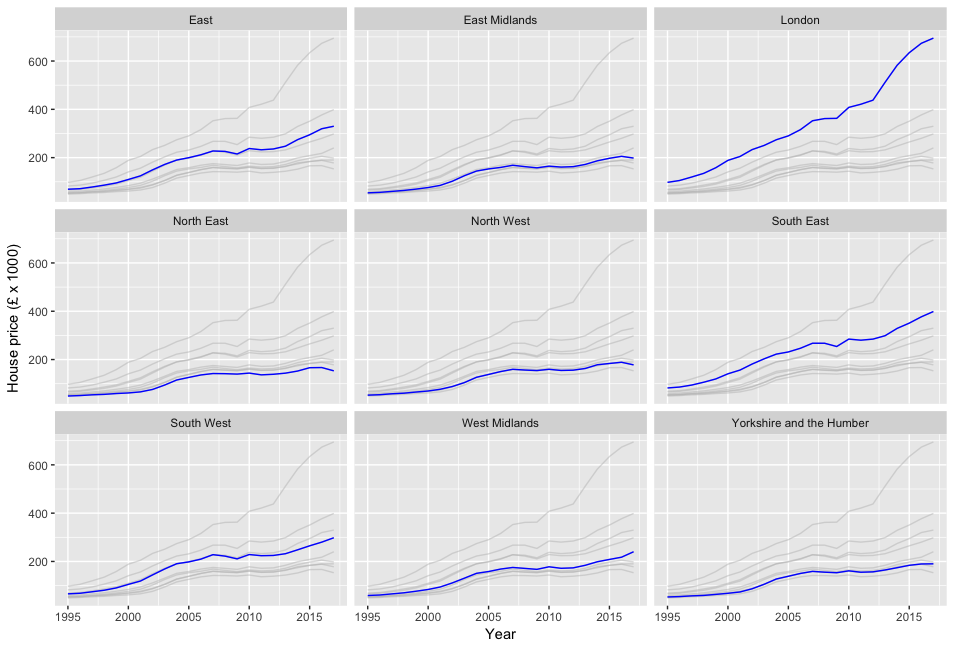
\includegraphics[width=1\textwidth]{house_prices_england.png}
\caption{House prices in England, 1995-2017}
\label{fig: house_prices}
\end{figure}

 An important consequence derived from these restrictions has been a substantial 
                  increase of the house prices. Figure \ref{fig: house_prices} 
     plots the evolution on time of the house prices across different regions in 
     England during the last two decades. In addition to London, the areas that 
     have registered greater increases are the South East, Esat and South West 
     respectively. 
  
  \section{Econometric framework}
  
  \subsection*{Main sources of data}
  
  
The data corresponding to  the sample of analysis in this paper cover years from 2011 to 2016 
  that we divide into three time intervals $t  (t = 1, 2, 3)$ that include March 2011 – March 2013, 
  March 2013 – March 2015 and March 2015 – September 2016. These data are 
  retrieved from several sources and are referreed to 324 local planning 
  authorities. We cluster our information at this level since these type of local authorities are likely to rule the housing planning policies and then 
  determine the house prices. Therefore we assume that each of those represents a local market and
  a unit for the analysis. 
  
  
   Our main goal consists of studying the effect of prices on entry of care 
   homes in the local market. In the spirit of \citet{tokunaga2013factors}, who analyse
 the choice local markets by private long term care providers in Japan, we proxy the entries as the proportion as the number
  of care homes per 1000 population in the local authority that
 are aged 65 or over. We obtain the information concerning the characteristics and dynamics of the
care homes from the Care Quality Commission (CQC) directory of active and inactive
care homes\footnote{This dataset is maintained by the CQC Directorate of Data and Statistics and available upon request.}
This dataset contains all the registrations of care homes that have carried out a regulated activity since
   2010. The initial sample includes 24,354 records. Our analysis is restricted to the entries from March
    2011 onwards since a substantive proportion of the total registrations (16,054) were 
     carried out during 2010 and the first two first months of 2011 as a result 
     of a new regulation.\footnote{Since October 2010 registration in Care Quality Commission  became a legal requirement for every long 
     term care provider who wanted to carry out a regulated activity.} As we illustrate in Figure \ref{fig: registrations}, this process 
     was prolonged for the remaining months of 2011 particularly until July. The forthcoming years presented  
     progressively a less intense level of registrations.
     
\begin{figure}[ht]
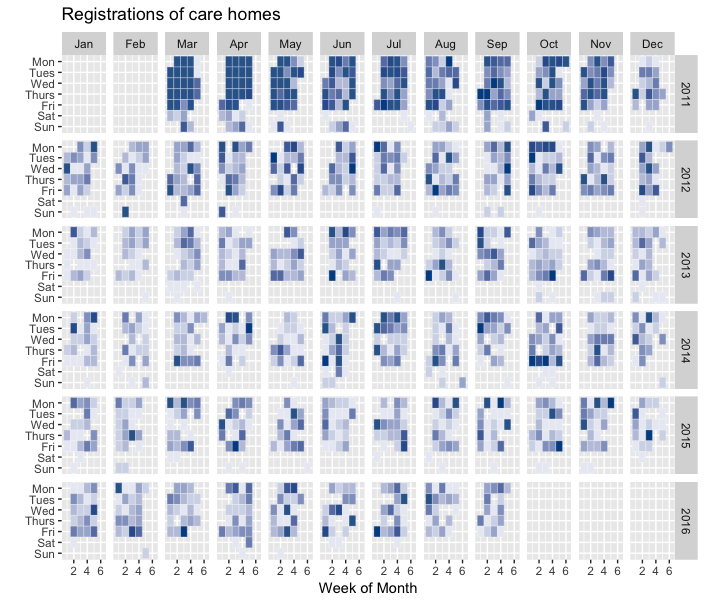
\includegraphics[width=1\textwidth]{registrations.png}
\caption{Care homes registrations in the CQC (2011- 2016)}
\label{fig: registrations}
\end{figure}

A major strength of this dataset for the purposes of this research consists of the opportunity 
to track the entries and exits of the care homes in the market. Besides, it provides further
 individual information regarding the care homes that includes 
the number of beds in the care home, the identifier code, the name of the care home, the postcode and postal 
address, the city and region where the care home is located as well as the local authority responsible for the 
social care activities corresponding to the location of the care home. Likewise, with the exception of the number of
 beds, the same information is available with regards to the providers where the care homes belong to. 
 
 In our analysis we only consider \textit{de novo} entries that represent the 
 beginning of a new activity and effectively the entry in the market. Neglecting these may
   introduce bias in the results. \citet{geurts2016firm}, for instance, analyse the effect of this measurement
            problem on the estimations of the firm’s growth after the entry in the 
            market.\footnote{In the Appendix \ref{appendix market_entries} we present further details about the computation of this variable}


In a second stage of our analysis we use information
corresponding to quality ratings derived from the system
implemented by the CQC since 2014. On the basis of five 
dimensions\footnote{These dimensions entail the evaluation of issues related to the safety, the effectivity, 
the level of care and response to people’s needs as well as the management of the services.}, this new approach
  set a systematic method for collecting evidence that enables a more consistent assessment and comparison
   of the care homes’ performance. Services are rated according to four categories: {\it outstanding, good, requires
    improvement or inadequate}. For our analysis we collapse these categories into two: bad (requires improvement 
    and inadequate) and good (outstanding and good). Because the information is only available since October 2014, this part of the analysis considers a different
   timeframe that involves three waves from October 2014 - May 2015, May 2015 – February 2016 and 
   February 2016 – September 2016. 
   
   Likewise we test the effect of the house prices on the level of 
    residential care expenditure for each local authority. We represent the level
 of public expenditure throughtout the yearly gross current expenditure per adults over 65.\footnote{This is a well established fiscal measure of 
 government spending and it represents the expenditure that is not offset by income from clients and does not include capital charges either. Gross current expenditure $G$
  is calculated as: $G = T - C$ where $T$ is Gross Total Expenditure and $C$ incorporates capital charges. 
  Likewise, $T$ is obtained from deducting incomes from joint arrangments $I$, the NHS $N$ and other incomes $O$ to the total expenditure
   $E$, $T = E - (I+N+O)$} For our analysis we select 
  information corresponding  to the report of years 2011/12 to 2015/16 released by the NHS Digital\footnote{Further details
   may be found in \href{https://www.digital.nhs.uk/article/219/What-is-NHS-Digital-}{https://www.digital.nhs.uk/article/219/What-is-NHS-Digital-}} (formerly the HSCIC). 
   
    The information corresponding to prices of the properties is obtained from the price paid dataset
    released on a monthly basis by the Land Registry. This dataset contains all the transactions of
     properties carried out in England and Wales since 1995.  In addition to the price paid for the transaction,
    the dataset includes further information such as the type of property, the address, the city, district
     and region where the property is located as well as other information such as whether it is newly built
     and whether the property is under leasehold or freehold. The information regarding the transactions is
     collected on a daily basis we are able to subset the information according to the pre-defined periods of
     analysis. Then we group transactions that belong to the same planning authority and retrieve the average 
     price of them. The final output consists of an average price for each local planning authority for each
    period of analysis. 
        
    Inspired by \citet{hilber2016supply}, our identification strategy exploits changes over time in the restrictiveness of the 
planning regulations. This variable is built considering a series of historical
  planning applications from the Department of Communities and Local Government (DCLG) 
  since 1978 and it is defined as the refusal of 10 dwellings or more per year. As we shall explain in further detail 
    below, this measure may be subject to endogeneity concerns. In order to correct for 
    these potential limitations, we use an alternative measure 
    of planning regulations, the rate in change of delay of major projects which is also obtained from the DCLG. We
    also use the variation in the historical 
    political composition of the local authorities. Using data from the British Election Studies Information System, 
    we capture a series of the historical Labour vote share at the General Election since 1983. 
    In order to control for possible bias of associated with the former, we 
    also include data on the most recent election corresponding to June 2015. 
    Data are obtained from the Parliament website platform.\footnote{Further information is provided  in the following link \href{http://www.data.parliament.uk/dataset/general-election-2015}{http://www.data.parliament.uk/dataset/general-election-2015}} 
    
    Finally our regressions also include a number of control variables 
    that represent various characteristics of the local markets where the care 
    homes enter. These variables are retrieved mainly from the Department of 
    Work and Pensions (DWP) and we provide a more detailed justification of 
    their choice in the following subsection.
    
 \begin{table}[ht]
\centering
\caption{Descriptive statistics}
\label{table descriptive statistics}
\resizebox{\textwidth}{!}{% 
\begin{tabular}{lrrrrr}
  \toprule
 & Obs & Mean & Minimum & Maximum & Stdev \\ 
  \hline
Care homes per 1000 population over 65 & 945 & 1.67 & 0.43 & 4.06 & 0.54 \\ 
  Average house price & 945 & 268564.40 & 91157.13 & 2170757.48 & 179557.85 \\ 
  Share of population 85+ & 945 & 0.00 & 0.00 & 0.01 & 0.00 \\ 
  Share of population receiving Attendance Allowance & 945 & 0.01 & 0.00 & 0.03 & 0.00 \\ 
  Share of population with pension credits & 945& 0.03 & 0.01 & 0.07 & 0.01 \\ 
  Share of female claiming for JSA & 945 & 0.00 & 0.00 & 0.02 & 0.00 \\ 
  Share of population with income support & 945 & 0.01 & 0.00 & 0.04 & 0.01 \\ 
  HHI & 945 & 0.03 & 0.01 & 0.49 & 0.04 \\ 
  Share of Labour voters 2015 & 945 & 0.28 & 0.07 & 0.73 & 0.14 \\ 
 Rate of refusal of major & 945 & 0.26 & 0.07 & 0.51 & 0.09 \\ 
  Rate of delay change & 945 & -0.04 & -0.63 & 0.53 & 0.22 \\ 
  Historical share of Labour voters & 945 & 0.16 & 0.00 & 0.41 & 0.09 \\ 
  Proportion of bad quality & 945 & 0.19 & 0.00 & 0.66 & 0.12 \\ 
  Proportion of good & 945 & 0.56 & 0.00 & 4.71 & 0.59 \\ 
  Average expenditure per capita & 945 & 41004.65 & 2067.00 & 131972.00 & 29378.64 \\ 
   \bottomrule
\end{tabular}}
\end{table}
    
 Table \ref{table descriptive statistics} shows descriptive statistics of the 
 main variables of our estimation sample.The information is presented at the level of local planning 
 authorities and we also include the sources of information employed. 
 On average, over the period of analysis (March 2013 – September 2016) 
 there were about 1.7 care homes per 1000 population over 65. 
 Yet, this proportion varied notably across the different local planning authorities 
 where some present less than 1 (0.4) care homes per 1000 population
  and some others more than 3.5 up to a maximum of 4.06. Other variables in Table \ref{table descriptive statistics} 
  also reflect this local variation in the market for long term care. 
  Interestingly there is a planning authority that registers a maximum
   average value for the houses of £2,170,757. Apart from this outlier, the average house prices is £268,764.
 
 \subsection*{Econometric specification}
 
 Our purpose is to test the effect of the house prices on the proportion of care homes in local
  long term care markets. Considering a local authority $i$ during a time period $t$, the proportion of care homes $C$ can be 
estimated with a simple regression model specified as follows
 
 \begin{eqnarray}
\label{eq: equation1}
   C_{it} = \beta X_{it} + \alpha P_{it} + \psi_{c} + \epsilon_{it}
 \end{eqnarray}

where $X_{it}$ represents a vector with different observable variables
 that characterize the composition of local long term care markets and that we use as controls. Hence, on the one hand
 we define the demand for long
  term care in the local market  by addressing a number of issues. Firstly, we include the proportion 
  of people older than 85 and proportion of people that receive the attendance 
  allowance\footnote{This benefit aims to support those people with physical disabilities in UK that live
   independently and might require residential care services otherwise. } as proxies of the level 
   of health dependency. Also, given the association between the financial needs and the funding
    support determined by the means-test, we incorporate the proportion of people that receive some
     sort of income support and the proportion of people that receive pension credits to reflect the payer 
     composition within the local population. These variables have been previously used in the literature for these purposes 
     \citep{darton2010slicing, forder2014}. Likewise, given that long term care is a labour intense activity,
      we add the proportion of females that claim for job seekers’ allowance in order to get a proxy for unemployment.
      
      In addition to the former, $X$ also includes a measure of the Herfindahl–Hirschman Index (HHI) to control for
      the competition between care homes in the local market. In our case, the HHI is a measure of concentration that 
      reflects the squared shares of beds across all the providers in a local market. The values range from
       0 to 1 where higher values represent higher concentration and therefore less competition.  We also include
       county fixed effects $ \psi_c$  associated with each local authority in 
       order to capture 
       
       $P_{it}$ is the average of the house prices and $\epsilon$
       represents an error term that is identically and independtly distributed. In this specification $\alpha$ is the 
       parameter of interest and thus is interpreted as the impact of house prices on the proportion 
       of care homes. Equation \ref{eq: equation1} can be estimated by OLS and will produce an unbiased estimate of $\alpha$ only if
         $P_i$ is exogenous so that $Cov(P_{i}, \epsilon_{i}) = 0 $ . In case this occurs, this estimate may be effectively interpreted as
          a causal effect. Nonetheless, as we argue below, there may be elements that violate the former and introduce correlation between $P_{it}$ and
 $\epsilon_{it}$ resulting in biased estimates of $\alpha$. We address this concern by using an instrumental
  variables (IV) approach and estimating the two-least squares estimator of $\alpha$. 
  
    \subsection*{Bias and specification}
   
A potential element that can lead to inconsistent estimations of $\alpha$ may be the presence of unobserved
 variables that confound the effect of the house prices and proportion of care homes. For example, one may think about
  the effect of unobserved incomes that may affect positively the values of the properties and also incentivise
   the entries in the market given likely wealth effects. Hence, higher level of housing prices may result in
    wealth effects that lead to greater levels of consumption and then attract businesses. Hence the selection
     of an area by a care home provider is likely to be non-random and the effect of $P_{i}$ may be associated partially 
     with $\epsilon$. In order to tackle with these potential
      problems, it is necessary to find an instrumental variable $z$  that is uncorrelated with $\epsilon$ but is correlated
       with $P_{i}$.
       
  The identification strategy for meeting this purpose is based on
  \citet{hilber2016supply}.
The main underlying idea of their strategy consists of exploiting variability of various supply
constraints associated with the local housing markets in England in order to explore the effects of local earnings
 on house prices. Their findings confirm the vision that tight supply regimes – e.g. with more regulatory 
 constraints in the planning regulations, lead to increases in the prices. In our case, we apply directly 
 the planning regulation instruments to the house prices. For our identification we assume that this instrument,
  in addition of being correlated with local earnings is also correlated with the house prices. 
  
  Both the relationship between planning regulations and house prices as well as the use of planning regulations 
  for addressing endogeneity bias associated with house prices have been well documented in the literature. 
  Considering the case of UK, several authors have shed light with regards to the effects of tight planning 
  regulations on house prices suggesting a positive relationship \citep{cheshire2009, cheshire2014, barker2004barker, hilber2016supply}
  
 Yet there is a remaining problem concerning the way developers perceive the planning regulations. 
One may question whether the behaviour of developers is modified when they are aware of the level
 of tightness of certain local planning authorities are tighter than others. It may happen that if they know
  that some local planning authorities are particularly restrictive they may deter their applications and focus
   on other markets. If this occurs, then the observed refusal rates may not reflect the level of real 
   restrictiveness, especially in the cases of more limiting local planning authorities. For coping with this
    limitation it is possible to exploit two identification strategies on the basis of \cite{hilber2016supply}.
    
     The first involves a planning reform aimed at speeding up the planning processes and the
      second links the planning regulations and the variation in the share of local political power. 
The main idea corresponding to the identification strategy based on the planning reform consists
 of exploiting the variation in the change in the delay rates before and after the reform. Set in 2002,
  the reform included the establishment of an explicit goal for major development projects. The main
   purpose of this target was to avoid the delays of major projects by local planning authorities. Despite
    they were not formally penalised for not meeting the target, local planning authorities did not have
     the incentive for neglecting the target either. The central government could retain financial resources
      addressed to local planning authorities. An option for local authorities to meet the target was to refuse 
      greater projects and conversely approve smaller projects which could be finished on time. 
      
On the basis of the former, it is possible to think on the behaviour of the local planning authorities
 before and after the reform paying particular attention to their level of restrictiveness. Thus, before 
 the reform local planning authorities that were more restrictive would be also the ones that had greater 
 delays and thereby the least likely to meet the target. Once the reform was established, these local 
 planning authorities would be also the ones more likely to refuse more projects and therefore suffer less
  delays. Less restrictive local planning would not have to alter their behaviour substantially.
   Considering this, we allow for a 10-year period to represent the average delay rates pre and post reform.
    Hence we consider the delay rates 1994 and 1996 and the delay rates between 2004-2006.  
    
Regarding the relationship of political power and the application of local planning regulations we take
 advantage of the variation in the political composition of the local council. In addition to 
 \citet{hilber2016supply},
  this strategy has been used by other authors such \cite{bertrand2002does}, \cite{sadun2015} or \cite{cheshire2016}.
  Hence, we use the share of Labour party votes at the General Election of 1983.
   The information is obtained from the British Election Studies Information System.  
   We choose the share of Labour voters since we believe that the attitudes of these voters 
   will be more inclined to grant house access rather than to preserve the value of the properties.
    Also, we could have used the results derived from local elections. 
    Yet, these might be correlated with the development of local housing markets and constitute a source
     of potential bias. The time frame of 1983 provides the earliest date where election results can be linked
      to data corresponding to local authorities and then minimizes the potential association between the
       outcome of the election and the planning process.
         
Considering these caveats, we specify equation \ref{eq: equation2} in order to estimate first-stage fitted values of the log
 house prices. The predicted values derived from this equation are used as instruments and incorporated in
 \ref{eq: equation1}in order to get a consistent estimate of $\alpha$.
 
  \begin{eqnarray}
\label{eq equation2}
   P_{it} = \delta Z_{it} + X\beta_{it} +  \psi_{c} + u_{it}
 \end{eqnarray}

where $Z$ are a set of observables that will be used as instruments. 
For the reasons discussed above, we employ the share of Labour voters and the 
changes in delay rates pre and post reform.  $X$ incorporates the same set of market controls included in \ref{eq: equation1}.

Table \ref{table first_stage} shows evidence on the validity of the instruments that we could consider for overcoming 
the endogeneity problems in our analysis. On te basis of the regression
specified in equation \ref{eq equation2}, the first column
provides the estimates referred to the relationship between the rate of refusal and the 
house prices.  The positive relationship between the level of regulatory tighhtness in the planning 
regulations and house prices is consistent with previous findings in the literature . Nonetheless, for the reasons exposed above the 
rate of refusal may suffer endogeneity so considering the regression with only this instrument would validate our results corresponding
to the second stage. Columns 2 and 3 present the estimates 
corresponding to the instruments proposed to tackle with this limitation - the 
change in the rate of delay and share of Labour voters respectively. The results of this first stage 
point at the direction that we would expect. Hence, the greater changes in the delay rates pre and
 post reform influence negatively the prices. In this case, these big differences would imply reductions in the rate of delay for restrictive
  local authorities which would be substituted with more rejections of the major projects and therefore 
  greater refusal rates. Likewise, the share of Labour voters is also associated with lower levels in the house prices. 
  

\begin{table}[h]
\centering
\caption{First stage results, dependent variable house prices (log)}
\label{table first_stage}
\resizebox{\textwidth}{!}{% 
\begin{tabular}{@{}lccc@{}}
\toprule

                                    &  & {Average house price (log) } & {}
 
                      &              & Refusal rate & {Change rate of delay } & {Share votes of Labour} \\ 
\hline
                & 1.222***   & -0.095           & -1.672***          \\
                                    & (0.28)     & (0.066)               & (0.328)              \\
\hline
Observations                        & 945                   & 945                    & 945                   \\
R2                                           & 0.694               &        0.672         &   0.695                    \\
F (excluded instruments)     & 19.42***     &          2.07              &     46.32***                  \\
\bottomrule
\end{tabular}}
\begin{tablenotes}
      \scriptsize
      \item {\it{Notes}}: All regressions include the following controls. Share of people 85+, 
      Share of people receiving Attendance Allowance, Share of people with pension credits, 
      Share of females claiming for Job Seekers Allowance, Share of adults with income 
      support, 
      Herfindahl-Hirschmann Index, share of Labour voters for 2015. All regressions include fixed effect controls at
      county level. Robust standard errors in parentheses. Standard errors are clustered at local planning 
      authority level. ***/**/*/$^{+}$ denote significance levels at 1\%, 5\%, 
      10\% and 15\%. Standard errors are presented in parentheses. 
    \end{tablenotes}
\end{table}

  According to the results derived from the F test of excluded instrument, we can conclude that $P_{i}$ 
  is weakly identified through the rate of delay change. Therefore we consider 
  the share of Labour votes as the preferred instrument. 
  
  As we introduced before a potential issue for the reluctance of this instrument may be related to 
unobserved trends. For instance, some areas have been exposed to the inflow of
certain residents that may changed the demographic composition of certain areas and this also modified the voting behaviour. In order to 
control for this we include the share vote for each local authority 
corresponding to the results of the last national elections celebrated in June 
2015.\footnote{ \citet{cheshire2016} use this instrument for analysing the effect of planning regulations on the 
proportion of vacant houses in England. They provide housing markets in Greater London as an example of areas
that could have changed  their voting behaviour as a consequence of these inflows.}

\section{Results}

\subsection{House prices and market entries}

Table \ref{table second_stage} reports the main results derived from the estimation regarding the impact 
of house prices on the proportion of care homes based on the second stage of our 
specification presented in equation \ref{eq: equation1}. The results in first column 
ignore the fact that prices may be subject to endogeneity and report OLS estimates that indicate 
and adverse association between the care home entries and the level of prices in 
the housing market. 

\begin{table}[h!]
\centering
\caption{Second stage results, effects of house prices on care homes entry}
\label{table second_stage}
\resizebox{\textwidth}{!}{% 
\begin{tabular}{@{}lllll@{}}
\toprule
                                    & \multicolumn{4}{c}{Care homes per 1000 people over 65}                                              \\ \midrule
                                    & \multicolumn{1}{c}{OLS} & \multicolumn{1}{c}{IV} & \multicolumn{1}{c}{OLS} & \multicolumn{1}{c}{IV} \\
\hline
Average house prices (log)                      & -0.111                  & 0.846*                &                         &                        \\
                                    & (0 .128 )              & (0.329)               &                         &                        \\
Average lagged house prices (log)             &                         &                        & -0.132            & 0.863**            \\
                                    &                         &                        & (0.127)                 & (0.33)               \\
\hline
Observations                        & 945                     & 945                    & 945                     & 945                    \\
R2                                  &                         & 0.1406                 &                         &                        \\
F statistic                         & 17.02***                &                        & 16.53***                &                        \\
\hline
Cragg-Donald Wald F statistic       &                         & 70.96                 &                         & 72.86                 \\
Kleibergen-Paap rk Wald F statistic &                         & 26.04                &                         & 29.12                 \\ 
\bottomrule
\end{tabular}}
\begin{tablenotes}
      \scriptsize
      \item {\it{Notes}} All regressions include the following controls. Share of people 85+, 
      Share of people receiving Attendance Allowance, Share of people with pension credits, 
      Share of females claiming for Job Seekers Allowance, Share of adults with income 
      support, 
      Herfindahl-Hirschmann Index, share of Labour voters for 2015. All regressions include fixed effect controls at
      county level. Robust standard errors in parentheses. Standard errors are clustered at local planning 
      authority level. ***/**/*/$^{+}$ denote significance levels at 1\%, 5\%, 
      10\% and 15\%. Standard errors are presented in parentheses. 
    \end{tablenotes}

\end{table}

The second column provides the estimates when we control for the endogeneity of the house pricesg by using
the Labour share of voters corresponding to each local authority.  Thereby, areas that have higher level of house prices
seem to attract care homes.  Hence, we find  that an increase 
of 100\% in the level of prices would supposed an increase of 0.84 care homes 
for 1000 population over 65.  Yet, this positive effect is significant at the 10\% level. 

One may argue that this effect is not correctly measured since the decision of 
entry in the market entails certain lags. For instance, providers may base their decision of entry in past house prices rather
than the existing in the market. Furthermore using contemporaneous prices may 
lead to  reverse causality issues. For the reasons outlined in previous sections, house prices may affect the entry of care 
homes. Analogously, care homes may be also an amenity in the area that may 
lead to an increase in the value of the properties located there. In order to 
tackle with these concerns, in columns three and four we present the results of the effects 
derived from house prices that are lagged two years. The effects are similar to 
the findings that we obtain while using contemporaneous house prices. Thus, the positive effect derived from the IV 
regression apart from being greater (0.86) is more significant at the 5\% 
level.

In any case, according to the results from the Kleibergen-Paap and the Cragg-Donald Wald 
statistics, potential objections regarding the weakness of the identification for both contemporaneous and lagged prices, do not seem to 
be an issue.  


\subsubsection*{\normalsize{\it Robustness checks}}
 
In order to test the robustness of our results, we run various models.
 Firstly, a plausible concern may be the presence of some outliers in
  the distribution of care homes. In order to overcome the potential influence 
  of these observations we remove from the sample the top and bottom 5\%  of the care homes.
 Likewise, we also consider a sample without the planning authorities belonging to the region of London.
   The results of these analyses are shown in Table \ref{table robustness}. It is important to highlight that the specifications 
   corresponding to each of the columns are identical to the specifications presented in Table 
   \ref{table second_stage}.
 
 
\begin{table}[h!]
\centering
\caption{Robustness checks, effects of house prices on care homes entry}
\label{table robustness}
\resizebox{\textwidth}{!}{% 
\begin{tabular}{@{}lllllllll@{}}
\toprule
                         & \multicolumn{2}{c}{OLS} & \multicolumn{3}{c}{IV}                          \\ \midrule
                         & No controls  & Controls & Change delay rate & Labour share & Labour share \\
                         & (1)          & (2)      & (3)               & (4)          & (5)          \\
Average prices (log)     & -0.2499***   & 0.0558   & -0.0535           & (0.2373)**   & $0.4160^{+}$ \\
                         & (0.0387)     & (0.1512) & (0.2195)          & (0.1206)     & (0.2755)     \\
Main controls            & No           & Yes      & Yes               & Yes          & Yes          \\
Local authority controls & No           & Yes      & Yes               & Yes          & Yes          \\
Additional controls      &              &          &                   & No           & Yes          \\
F                        & 41.73***     & 26.49*** &                   &              &              \\
R2                       & 0.0424       & 0.2131   &                   &              &              \\
Observations             & 945          & 945      & 945               & 945          & 945          \\ \bottomrule
\end{tabular}}
\begin{tablenotes}
      \scriptsize
      \item {\it{Notes}}:All regressions include the following controls. Share of people 85+, 
      Share of people receiving Attendance Allowance, Share of people with pension credits, 
      Share of females claiming for Job Seekers Allowance, Share of adults with income 
      support, 
      Herfindahl-Hirschmann Index, share of Labour voters for 2015. All regressions include fixed effect controls at
      county level. Robust standard errors in parentheses. Standard errors are clustered at local planning 
      authority level. ***/**/*/$^{+}$ denote significance levels at 1\%, 5\%, 
      10\% and 15\%. Standard errors are presented in parentheses. 
    \end{tablenotes}

\end{table}


The results from Table \ref{table robustness}  confirm the consistency of the baseline results. 
As shown in Figure \ref{fig: house_prices} London reported the greatest 
increase in housing prices during the last two decades. The influence of those local authorities 
belonging to London is shown by a positive and higher but less significant 
effect of the house prices on the entry of care homes. Hence, an 100\% increase of the 
house prices leads to increases of 1,6 and 1,5 care homes depending on the 
whether the house prices are correspond to the existing period of time or 
conversely are lagged. 

The presence the outliers, as represented by the top and bottom 5\% of our sample appear to 
have some influence in the results. Considering columns 5 to 8 in Table \ref{table robustness} 
the effect of house prices on the entry of care homes in addition of being positive, even for the OLS 
estimates, is significant at 5\% level. 

In general, these findings suggest that providers would be focusing
 on more affluent areas possibly aiming at securing potential clients that do not rely on public funding 
 arrangements. A reason for this may be the aim of providers for minimizing the effect derived
  from the existing cross-subsidisation from self-funded to publicly funded clients. 
  \citet{humphries2016social} argue that this strategy has been followed by a number of long term
   care providers in order to preserve their financial viability and overcome the funding 
   crisis. In the next section we investigate further mechanisms that may 
   explain the effects  reported in Tables \ref{table second_stage, table 
   robustness}.

\subsection{Exploration of further channels}

\subsubsection*{\normalsize{\it Effect on the social care expenditure}}

The positive effect of prices on the entry of care homes may be indicative of a transfer in the demand from the public to the self funded
clientele. Next we test the effect of the house prices on the level of per capita expenditure in 
residential care. Rather than the whole adult population, we restrict our analysis to the 
population who is 65 or more since this is the segment of population more likely 
to demand these services. 

\begin{table}[h!]
\centering
\caption{Second stage results, effects on per capita expenditures}
\label{table expenditure}
\resizebox{\textwidth}{!}{% 
\begin{tabular}{@{}lllll@{}}
\toprule
                                    & \multicolumn{4}{c}{Per capita expenditure on residential care}                                      \\
                                    \hline
                                    & \multicolumn{1}{c}{OLS} & \multicolumn{1}{c}{IV} & \multicolumn{1}{c}{OLS} & \multicolumn{1}{c}{IV} \\
\hline
Average house prices (log)                        & -0.153                 & $-0.725 ^{+}$               &                         &                        \\
                                    & (0.122)               & (0.483)             &                         &                        \\
Average lagged house prices (log)                &                         &                        & -0.197                 & $-0.74 ^{+}$               \\
                                    &                         &                        & (0.128)               & (0.484 )            \\
\hline
Observations                        & 945                     & 945                    & 945                     & 945                    \\
R2                                  & 0.8604                  &                        &                         &                        \\
F statistic                         & 103.88***               &                        & 103.59***               &                        \\
\hline
Cragg-Donald Wald F statistic       &                         & 70.959                 &                         & 72.864                 \\
Kleibergen-Paap rk Wald F statistic &                         & 26.039                 &                         & 29.122              \\  
\bottomrule
\end{tabular}}
\begin{tablenotes}
      \scriptsize
      \item {\it{Notes}}:All regressions include the following controls. Share of people 85+, 
      Share of people receiving Attendance Allowance, Share of people with pension credits, 
      Share of females claiming for Job Seekers Allowance, Share of adults with income 
      support, 
      Herfindahl-Hirschmann Index, share of Labour voters for 2015. All regressions include fixed effect controls at
      county level. Robust standard errors in parentheses. Standard errors are clustered at local planning 
      authority level. ***/**/*/$^{+}$ denote significance levels at 1\%, 5\%, 
      10\% and 15\%. Standard errors are presented in parentheses. 
    \end{tablenotes}

\end{table}

The  results derived from Table \ref{table expenditure} are in line with what should be expected. The negative 
 effect of house prices on the expenditure per capita is the result of the 
 inclusion of the property value in the means test. Higher values of the 
 properties reduce the elegibility for being publicly funded. Also, the low 
 significance may be explained by the fact that in these local authorites there 
 may be a fewer proportion of people that actually demand these public support. 

\subsubsection*{\normalsize{\it Effect on the distribution of care homes per level of quality}}

An alternative channel can be the distribution of care homes by their level of 
quality. In Table \ref{table quality} we show the results derived from the effect of house 
prices on this distribution. We can see that the effects are to greater extent more pronounced in the case of care 
homes of better quality although in any case these effects are not significant.

\begin{table}[ht]
\centering
\caption{Second stage results, effects on distribution of care homes by quality}
\label{table quality}
\resizebox{\textwidth}{!}{% 
\begin{tabular}{@{}lcccccccc@{}}
\toprule
                                    & \multicolumn{4}{c}{Good quality care homes} & \multicolumn{4}{c}{Bad quality care homes} \\ \midrule
                                    & OLS           & IV          & OLS           & IV          & OLS           & IV          & OLS           & IV         \\
\hline
House prices                        & 0.144*       & 0.189       &               &             & 0.06**      & 0.02      &               &            \\
                                    & (0.086)       & (0.24)      &               &             & (0.018)        & (0.06)      &               &            \\
Lagged House prices                 &               &             & 0.138+       & 0.193      &               &             & 0.04*       & 0.02     \\
                                    &               &             & (0.09)        & (0.246)      &               &             & (0.02)        & (0.061)     \\
\hline
Observations                        & 945           & 945         & 945           & 945         & 945           &             & 945           &            \\
R2                                  & 0.2942        &             & 0.2936        &             & 0.4379        &             & 0.432         &            \\
F statistic                         & 12.34***      &             & 11.91***      &             & 21.25***      &             & 20.72***      &            \\
\hline
Cragg-Donald Wald F statistic       &               & 70.959      &               & 72.864      &               & 70.959      &               & 72.864     \\
Kleibergen-Paap rk Wald F statistic &               & 26.039      &               & 29.122      &               & 26.039      &               & 29.122     \\ \bottomrule
\end{tabular}}
\begin{tablenotes}
      \scriptsize
      \item {\it{Notes}} All regressions include the following controls. Share of people 85+, 
      Share of people receiving Attendance Allowance, Share of people with pension credits, 
      Share of females claiming for Job Seekers Allowance, Share of adults with income 
      support, 
      Herfindahl-Hirschmann Index, share of Labour voters for 2015. All regressions include fixed effect controls at
      county level. Robust standard errors in parentheses. Standard errors are clustered at local planning 
      authority level. ***/**/*/$^{+}$ denote significance levels at 1\%, 5\%, 
      10\% and 15\%. Standard errors are presented in parentheses. 
    \end{tablenotes}
\end{table}

\section{Conclusion}

In this study we have investigated whether the high prices in the English housing market respresent a barrier to
 the provision of long term care services or contrarily they provide an incentive for care homes to set their 
 services. First, we test for simple OLS regression and we show that there are empirical constraints that produce
  biased estimates. Consequently we address these concerns by considering different variables associated with
    planning regulations to instrument the house prices. According to our findings, the use of the share of political
     power performs as a better instrument for addressing potential endogeneity concerns related to house prices.
       
       The results then suggest that house prices are positively associated with the entries and providers might
        therefore be driven to set their businesses in places where the prices of the properties higher. We explore 
        the underlying mechanism of this effect by examining how house prices affect the number of care 
        homes according to their quality rating. In sum, the positive effect of house prices on the entry of care
         homes is greater in cases where care homes have a better overall rating. A further avenue for this research
          could consider each of the dimensions involved in the quality inspections. 
          
Our results also point out at the connection between the housing market and the
 market of long term care activities. The coordination between local authorities at
  both county and district level is therefore encouraged to facilitate the provision of 
  further evidence about the relationships between both types of markets. 
  
\newpage
\bibliographystyle{apalike}
\bibliography{ex1}
%remember to use \citep{} for citation

\newpage
\end{document}

